\documentclass[10pt,journal,compsoc,draftclsnofoot]{IEEEtran}

% Definition of \subparagraph
\makeatletter
\newcommand\subparagraph{%
  \@startsection{subparagraph}{5}
  {\parindent}
  {3.25ex \@plus 1ex \@minus .2ex}
  {0.75ex plus 0.1ex}
  {\normalfont\normalsize\bfseries}}
\makeatother

\newcounter{subparagraph}[paragraph]

\usepackage{listings}
\usepackage{titlesec}
\usepackage{float}
\usepackage{hyperref}
\usepackage{array}
\usepackage{tocloft}
\usepackage{lscape}
\usepackage{textcomp}
\usepackage{pgfgantt}
\usepackage{amsmath}

\usepackage{geometry}
\geometry{margin=0.75in}

\setcounter{tocdepth}{4}
\setcounter{secnumdepth}{4}

\begin{document}
\onecolumn

\begin{titlepage}
\null
\vspace{15mm}

\begin{flushleft}
\begin{bfseries}
	\vskip2mm
	\Huge{Midterm Progress Report for\\ Better Graphics For A Robotics Grasping GUI}\\
	\vspace{15mm}
	\textbf{\huge Shady Robots} \\
	\vskip2mm
	\large{Group 12}
	\vskip5mm
	\Large{Justin Bibler \\
	Matthew Huang \\
	Daniel Goh \\}
\end{bfseries}

\vspace{15mm}
\Large{CS463: Senior Software Engineering Project} \\
\Large{Spring 2017} \\

\vspace{5mm}

\today

\vfill

\begin{normalsize}
{\bf Abstract:}
This document goes over the project our project's purpose and goal, as well as providing an update on our team's progress with the project.

{\bf Keywords:} OpenRAVE, shaders, warm cool shading, silhouettes, shadows, robotic simulation, geometry, visualization, render, ubuntu, vmware, virtualbox
\end{normalsize}
\end{flushleft}

\newpage

\end{titlepage}

\begin{flushleft}

\section{Project Purpose and Goals}
The purpose of our project is to update the graphics of an existing program that creates a simulation of a robotic arm grasping objects.
The reasoning behind our desire to update the graphics is because our client is using online data collection methods using these visualizations.
However, the outdated graphics are making it difficult for users to give confident responses to the survey.
To fix this problem, we have created 4 major goals:
\begin{enumerate}
\item Implement Gooch shading.
\item Implement shadows.
\item Implement silhouettes.
\item Test to ensure our implementations improve user confidence using interviews.
\end{enumerate}

\section{Where we are in the project}
The three required features: warm cool shading, shadows, and silhouettes, are completed.
Our team was also able to have a client evaluation session to receieve feedback regarding our implementations.
Changes were made based on our client's feedback, and the implementations were approved by our client.
Our team also ran a survey to determine if our team's implementation improved the users understanding of the visual, and we received good feedback based on the survey responses.
Further information regarding the survey data is located in the "Problems and Solutions" section under "Data Tabulation and Results".

\section{What is left to do}
As the three required features are completed, we will support the client whenever change or help is needed in regards to the graphics of OpenRAVE.

\newpage

\section{Problems and Solutions}
\subsection{Justin Bibler}
\textbf{Problem1}
\par
placeholder placeholder placeholder placeholder placeholder placeholder
placeholder placeholder placeholder placeholder placeholder placeholder
\par
placeholder placeholder placeholder placeholder placeholder placeholder
placeholder placeholder placeholder placeholder placeholder placeholder
\par
placeholder placeholder placeholder placeholder placeholder placeholder

\newpage

\subsection{Matthew Huang}
\par
By the end of our beta release, we had implemented warm cool shaders, silhouettes, and shadows together.
As a reminder, this required 2 render passes since the silhouettes need to be rendered separate from the other shaders.
Additionally, due to API limitations, we had to inject the warm cool shader code into the SoShadowGroup library so that the shadows would not override the augmented warm cool colors.
At this point, we were feature complete and all that was left to do was polishing based on client feedback.
When we demoed the project to Cindy, she suggested that we make alterations to each feature so that they were all more consistent across examples.
Specifically, she wanted the warm cool colors to adapt based on object color, more consistent silhouette widths across different shapes, and darker shadows.
Since I am responsible for the warm cool shaders and silhouettes, I will outline how those features were repolished; I will leave the darker shadows for Justin to explain.
Do note, however, that Justin and I largely colaborated in implementing all 3 feature changes.
\vspace{3mm}

\textbf{Adapative Warm Cool Shaders}
\par
To implement the warm cool color adaptation, we set color ranges that would catch each different object color we wanted to account for.
The colors we ended up accounting for were red, green, blue, yellow, purple, cyan, white, and grey/black.
After we caught one of the colors, we would then set specific warm cool colors that would blend well with object color.
For example, the warm cool colors for red are yellow and red respectively while the warm cool colors for green are green and blue respectively.
This allowed the scene to retain much of its original colors while also having the warm cool color ranges.
Additionally, this prevented bad color combinations such as blue and orange.
\vspace{3mm}

\textbf{More consistent Silhouettes}
\par
For the more consistent silhouettes, we found that the solution was to render the silhouette using polygonal lines (GL\_LINES) instead of solid polygons.
By doing this, every shape in the scene would have its own silhouette who's width was based on the set line width.
Then, changing the line width was simple; all we had to do was increase the line width value within our draw style module.
Additionally, to fix the silhouette overlapping issue, we also added a polygonal offset module to our silhouette render. 
This prevented the silhouettes from being at the same depth as the warm cool shaded model so any overlapping issue was largely resolved.
Also note that front and back face culling for the warm cool render and the silhouettes respectively were still being done.
Finally, the final silhouette color we choose was black.
This was our choice, despite the fact that they blended into the background, because silhouette are meant to simply help differentiate objects from each other.
\vspace{3mm}

\newpage

\textbf{Testing Performance}
\par
While implementing silhouettes, we ran into a line width runtime error that was causing our line widths to be immutable meaning our line widths would be stuck at 1.
What was interesting, though, was that this error only occurred while running the simulation on Justin and Daniel's machines, not mine.
What we found was that our virtual machines were accessing our laptop's hardware differently.
Namely, there's was using 3D hardware acceleration while mine was not.
Turning this option off fixed the line width problem, but hurt our program's performance.
Specifically, it dropped our frames per second from around 30-40 fps to 10 fps.
Our intuition told us that this was caused by our virtual machines being unable to properly use all of the hardware on our laptops.
To fix this, we had to install Ubuntu 16.04 natively on one of our laptops.
We switched to 16.04 from 14.04 because 14.04 had driver issues that prevented us from being able to access the internet.
This fixed our fps issues (now sitting at around 40 - 50 fps average) while still retaining the mutable line widths for our silhouettes.
\newpage

\subsection{Daniel Goh}
\textbf{OpenRAVE Performance Dropped With Our Implementations}
\par
With warm cool shading, shadows and silhouettes implemented, the performance for OpenRAVE simulation dropped significantly within our development environment.
The environment that was used during the development period was Ubuntu 14.04 on VMWare Workstation 12.
Barebones OpenRAVE run with 40 frames per second, however, with the implementations, the framerate dropped to 10 frames per second.
The source of the problem comes from using VMWare as it was not able fully utilize our machine's hardware.
This also caused graphical glitches to our silhouette implementation, causing the line width of silhouettes to not be changeable. 
\vspace{3mm}

We attempted to fix this problem by migrating our development environment to Virtualbox, which is another Virtual Machine Player.
This fix was able to solve the line width problem, however, the OpenRAVE simulation still runs poorly at around 10 frames per second.
The next fix that was attempted was to install Ubuntu 14.04 natively on our machines.
This attempt failed as Ubuntu 14.04 was not able to correctly detect the proprietary Broadcom Wireless driver.
This hindered our team from accessing required files for development from the internet.
Ubuntu 14.04 was also upgraded to the latest version, however graphical glitches such as flashing was introduced within the OpenRAVE simulation.
\vspace{3mm}

The attempted fix that solved all the problems was by installing Ubuntu 16.04 natively on our machines.
This solved the wireless issue, and essentially, OpenRAVE's performance issue as Ubuntu 16.04 was able to fully utilize the machine's hardware.
With proper use of hardware, the OpenRAVE simulation is able to run at around 50 frames per second.
This environment will be used to showcase our implementations during the Engineering Expo.

\newpage

\textbf{Creating the Survey}
\par
As warm cool shading, shadows and silhouettes are implemented, we needed to run a survey to determine if our implementations improve the user's understanding of the scene within OpenRAVE.
Early versions of the survey was designed to test if the user understands the scene.
This include questions that ask the relativity of objects with the scene and how they are positionally related to each other.
One of the questions tests the user's understanding of the scene by asking the position of the light source.
This version of the survey however, is not very insightful as the survey was too focused on testing the user's understanding without taking into account of the data tabulation methods.
This survey would only give us unsubstantial data results that is convoluted, and hard to tabulate.
And ultimately, this version of the survey would not aid us in determining if our implementations were able to meet its' goals.
\vspace{3mm}

To fix this problem, they survey was revised multiple times.
The new survey is updated to ask questions regarding the position of objects in the scene between the untouched and updated OpenRAVE visuals.
The new survey that was created also made use of Qualtrics blocks to separate survey questions into multiple pages.
This allows the survey to be created such that users are able to first answer the questions in regards to the untouched OpenRAVE visuals.
After they have completed their answers, they would be brought to another page with the same questions, but with the updated OpenRAVE visuals.
The aim of the new survey's structure is to test if users are able to answer the questions correctly with the untouched OpenRAVE visuals, and to test if they perform better in the survey questions with the updated OpenRAVE visuals.
\vspace{3mm}

This version of the survey was presented to our client (Cindy Grimm) for feedback and validation before we run the survey.
As the client is well-versed in running online surveys, especially in terms of Human-Computer Interaction, she provided some thoughts and advice to improve the survey.
The main addition to the survey was to question the users on their confidence levels, as with this data, we would be able to know if the users could better understand the scene.
The addition of the confidence questions were added after each question that tests the participant's understanding of the scene.
This data is tabulated and is used to inform us if our implementations were able to improve the confidence levels of users when answering the questions.

\newpage

\textbf{Data Tabulation and Results}
\par
As the survey is created and published using the Qualtrics survey platform, tabulating the data is simple as there are internal tools that is provided by Qualtrics for data analysis.
To summarize the data that we have gained, bar charts were created to easily visualize the collected responses from the survey.
The results that is shown is tabulated based on the data collected as of this writing (May 12, 2017).
As a quick rundown, the data that we have collected tells us that our warm cool shading, shadows, and silhouettes were able to improve the overall confidence levels of users when asked positional or scene related questions.

\begin{figure} [H]
  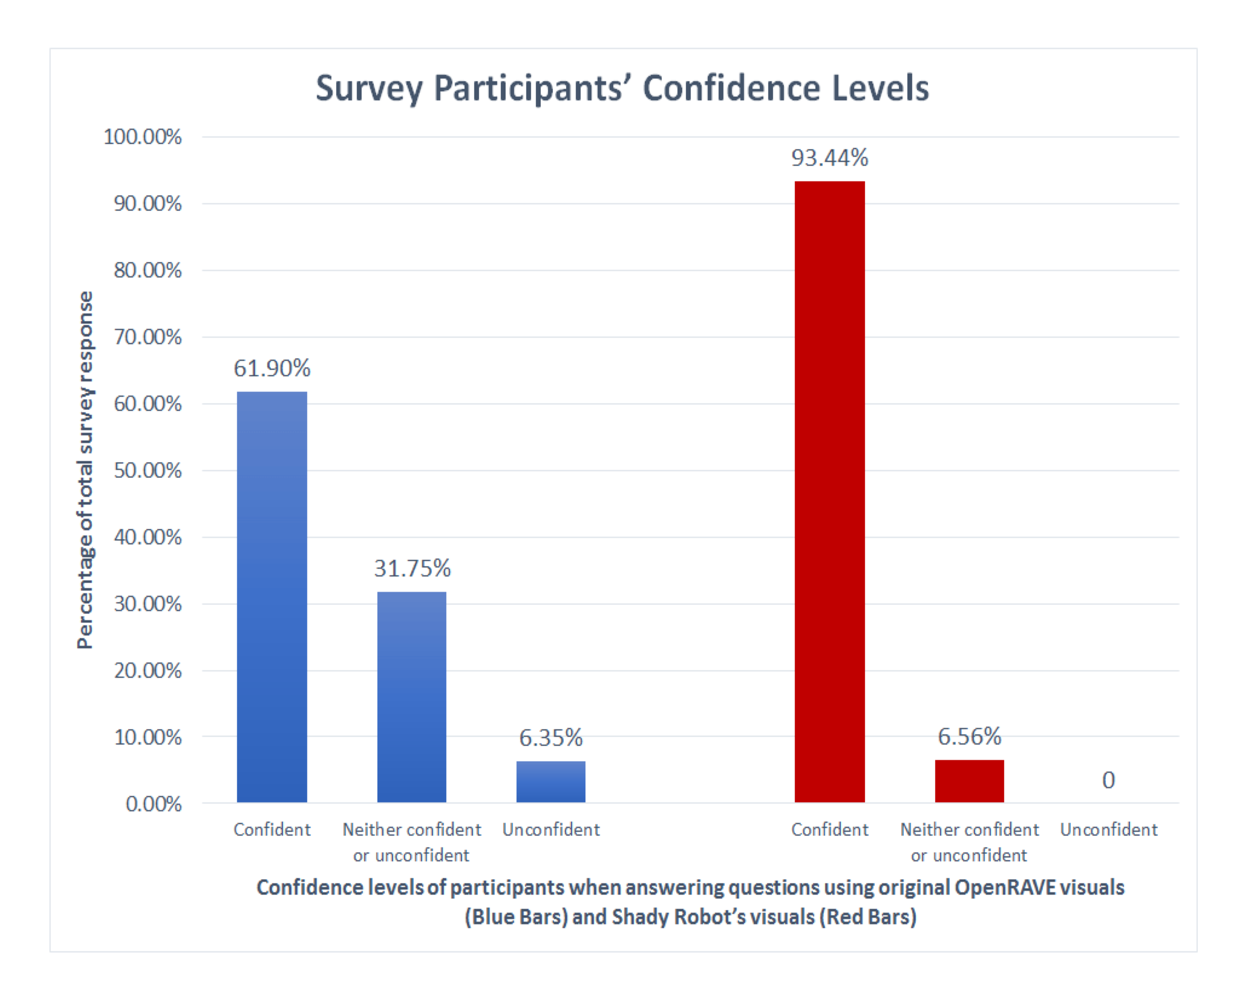
\includegraphics[scale=0.8]{ConfLevel.eps}
  \caption
{ \newline \hspace{\linewidth}
Bar chart showing the percentage of confidence levels when answering questions regarding his/her understanding towards the original visuals (blue bars) and the updated visuals (red bars) in our survey. The data above shows an increase in confidence levels when answering questions using the updated visuals.}
  \label{fig:Shadow}
\end{figure}

In addition to the improvement of overall confidence, 75\% of responses indicated that our implementation was able to added clarity to the scene.
Also, 65\% of the total response indicated that our implementation was more aesthetically pleasing.

\end{flushleft}

\end{document}

